\chapter{Machine Learning on RE}
RE are big part of language realization of a navigation system and especially so in the GIVE scenario. Part of my work was attempt to apply machine learning techniques on S-GIVE dataset with a clear goal to help navigation system with RE. This part is presented in this chapter.

In the first section I'll describe attempts at predicting timing of the first reference to a target button. Second section talks about modeling of chains of references.

\section{Introduction}
\section{Timing of the first reference}
Work of \citet{stoia2006sentence} was previously mentioned in related work section of chapter \ref{chap:bg}. They applied machine learning on timing of the first reference in a 3D virtual world. The set-up of their experiment is quite similar to the GIVE's one and so I decided it would be interesting to replicate their methodology on GIVE dataset. 

I defined the problem of the timing of the first reference as a classification task, as did \citet{stoia2006sentence}. More precisely binary classification, the two classes being either refer to the target button or delaying the reference. After extracting the first references to buttons which needed to be pressed from dataset, I excluded plural references, because of their complexity. Some buttons were placed on top of each other and IG wasn't sure which one need to be pressed. These were excluded as well because of the unnecessary confusion. That left me with 351 first references. For each first reference I have chosen one negative example, where IG could refer to the target but chose not to. I picked negative examples randomly from interval between entering room and time of the first reference. Overall, that is 702 data-points with perfectly balanced classes.

As for features extraction, I have chosen similarly to \citet{stoia2006sentence} various spatial information. For the positive examples, I averaged these spatial information over 0.6 seconds window centered on the time of the reference. Reasoning for that, is that IG take scene situation into consideration before and possibly after they start uttering the reference. All features are listed in following list. The list also includes figures' numbers. These figures are histograms of the attributes for positive and negative cases and can be found in Appendix.

\begin{itemize}
\item
Distance to target button - Figure \ref{fig:fref-distrib-dist}
\item
Absolute value of angle to target - Figure \ref{fig:fref-distrib-angle}
\item
Whether target is visible (True/False) - Figure \ref{fig:fref-distrib-visib}
\item
Number of distractors - Figure \ref{fig:fref-distrib-distractors}
\item
Number of distracting buttons - Figure \ref{fig:fref-distrib-distbuttons}
\item
Number of visible buttons with smaller angle to IF than the target button - Figure \ref{fig:fref-distrib-distangles}
\end{itemize}

Once I have extracted these features I have used three machine learning techniques: C4.5 decision tree because of their easy interpretation, naive Bayes to observe effect of all attributes and Support vector machine for linear classification. I used Weka software implementation of previous algorithms \citep{hall2009weka}.

For all the algorithms I used a standard ten-fold cross validation. The results can be seen in table \ref{tab:firstref}. Pruned decision tree for timing of the first reference can be seen in figure \ref{fig:dectree}. I used two simple baselines to compare the results with. I have perfectly balanced classes so the first baseline is 50\%. Simple rule for the first reference is to refer when the target is visible, and delay it if the target is not visible. In my case that rule has an accuracy of 64.2\%. 

\begin{table}[h!]
\begin{tabular}{lr}
\toprule
Model    & Accuracy (\%)  \\
\midrule
Class baseline    & 50.00\\
Visibility baseline & 64.2\\
\midrule
Naive Bayes  & \textbf{64.70} \\
C4.5 & 63.31 \\
SVM & 55.42 \\
\bottomrule
\end{tabular}
\caption{Results of first reference timing modeling}
\label{tab:firstref}
\end{table}

Only one algorithm was able to get over visibility baseline and not by a significant amount. These results were surprising, because \citet{stoia2006sentence} had success with the same approach on a similar dataset. Reasons for this difference are probably in the differences between their experiment and GIVE set-up. First, their tasks also included different actions than pushing buttons (e.g. picking up items). Second, their worlds had higher diversity of the distractors and smaller frequency of them. With increasing number of distractors and particularly distractors of the same category, it seems that spatial features loose their power in predicting the timing of the first reference. The number of visible distractors was the best attribute in their decision tree, but in my tree (figure \ref{fig:dectree}) it had lower information gain and moreover the tree did the split on number of visible buttons not of all distractors.

After the timing of the first references classification proved to be more difficult than excepted, I have switched from timing of the references to their content. I focused on chains of references.

\begin{figure}[h!]
\centering
\small
\begin{verbatim}
Distance to target <= 4.45
| Is target visible? = False: DELAY
| Is target visible? = True
| | Distance to target <= 2.51: REFER
| | Distance to target > 2.51
| | | Number of distracting buttons <= 4.67: REFER
| | | Number of distracting buttons > 4.67: DELAY
Distance to target > 4.45: DELAY
\end{verbatim}
\caption{Decision tree for first reference timing}
\label{fig:dectree}
\end{figure}

\section{Chains of references}
Section \ref{sec:dataset-chains} introduced the phenomenon of chains of references. It also analysed various linguistic functions, the chains can play in REG. This section will build on top of this analysis, by employing machine learning techniques to model the chains.

Valid and important question is whether chains aren't something, which should actually be avoided, instead of modelled. That is, what is the relation between usage of chains and task performance measure, such as duration. To address this issues, I used linear regression predicting the duration of the experiment explained by the average chain length. Figure \ref{fig:chains_dur_scatter} does contain a hint of a trend, but also contains many outliers. 

\begin{figure}[!htbp]
  \centering
	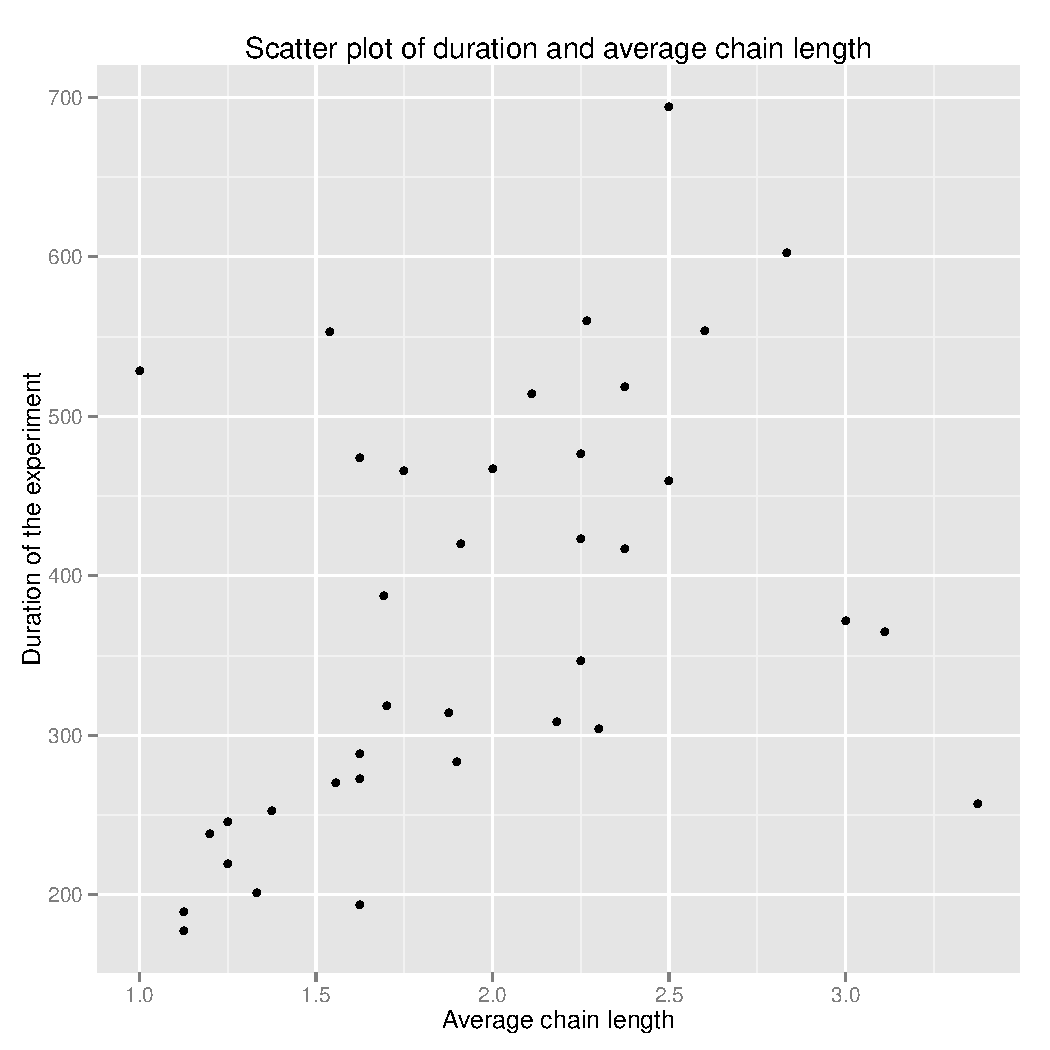
\includegraphics[width=0.8\textwidth]{Images/chains_duration_LR}
	\caption{Scatter plot of duration and chain length}
	\label{fig:chains_dur_scatter}
\end{figure}

When I applied linear regression the $R^2$ was 0.188, which means the average chain length explains very little of the duration variation. Correlation between the duration and average chain length is not so low: 0.433, however correlation does not imply causation. Longer chains can be caused by errors of IF or IG and the errors are likely to increase the duration. Based on these facts, I don't believe the chains are harmful phenomenon and it makes sense to proceed with attempting to model them. 